%%%%%%%%%%%%%%%%%%%%%%%%%%%%%%%%%%%%%%%%%
% a0poster Portrait Poster
% LaTeX Template
% Version 1.0 (22/06/13)
%
% The a0poster class was created by:
% Gerlinde Kettl and Matthias Weiser (tex@kettl.de)
% 
% This template has been downloaded from:
% http://www.LaTeXTemplates.com
%
% License:
% CC BY-NC-SA 3.0 (http://creativecommons.org/licenses/by-nc-sa/3.0/)
%
%%%%%%%%%%%%%%%%%%%%%%%%%%%%%%%%%%%%%%%%%

%----------------------------------------------------------------------------------------
%	PACKAGES AND OTHER DOCUMENT CONFIGURATIONS
%----------------------------------------------------------------------------------------

\documentclass[a0,portrait]{a0poster}

\usepackage{multicol} % This is so we can have multiple columns of text side-by-side
\columnsep=50pt % This is the amount of white space between the columns in the poster
\columnseprule=3pt % This is the thickness of the black line between the columns in the poster

\usepackage[svgnames]{xcolor} % Specify colors by their 'svgnames', for a full list of all colors available see here: http://www.latextemplates.com/svgnames-colors

\usepackage{times} % Use the times font
%\usepackage{palatino} % Uncomment to use the Palatino font

\usepackage{graphicx} % Required for including images
\graphicspath{{figures/}} % Location of the graphics files
\usepackage{booktabs} % Top and bottom rules for table
\usepackage[font=small,labelfont=bf]{caption} % Required for specifying captions to tables and figures
\usepackage{amsfonts, amsmath, amsthm, amssymb} % For math fonts, symbols and environments
\usepackage{wrapfig} % Allows wrapping text around tables and figures

\begin{document}

%----------------------------------------------------------------------------------------
%	POSTER HEADER 
%----------------------------------------------------------------------------------------

% The header is divided into two boxes:
% The first is 75% wide and houses the title, subtitle, names, university/organization and contact information
% The second is 25% wide and houses a logo for your university/organization or a photo of you
% The widths of these boxes can be easily edited to accommodate your content as you see fit

\begin{minipage}[b]{0.75\linewidth}
\veryHuge \color{NavyBlue} \textbf{Finding the centre:} \color{Black}\\ % Title
\Huge\textit{ correctioning asymmetry in high-throughput sequencing data}\\[2cm] % Subtitle
\huge \textbf{Jia R. Wu, Jean Macklaim, Briana L. Genge, Gregory B. Gloor}\\[0.5cm] % Author(s)
\huge The University of Western Ontario, Department of Biochemistry\\[0.4cm] % University/organization
\Large \texttt{ggloor@uwo.ca : ggloor.github.io : github.com/ggloor/ALDEx2}\\
\end{minipage}
%
\begin{minipage}[b]{0.25\linewidth}
\includegraphics[width=20cm]{/Users/ggloor/Documents/LaTeX/branding/one_logo.pdf}\\
\end{minipage}

\vspace{0cm} % A bit of extra whitespace between the header and poster content

%----------------------------------------------------------------------------------------

\begin{multicols}{2} % This is how many columns your poster will be broken into, a portrait poster is generally split into 2 columns

%----------------------------------------------------------------------------------------
%	ABSTRACT
%----------------------------------------------------------------------------------------

\color{Navy} % Navy color for the abstract
\vspace{-1cm}
\begin{abstract}
\large High throughput sequencing (HTS) generates millions of reads of genomic data regarding a study of interest, and data from high throughput sequencing platforms are count compositions. Subsequent analysis of such data yields information on transcription profiles, microbial diversity, or even relative cellular abundance in culture. Because of the high cost of acquisition, the data are usually sparse, and always contain far fewer observations than variables. However, an under-appreciated pathology of these data are their often unbalanced nature: i.e, there is often systematic variation between groups simply due to presence or absence of features. This variation is important to the biological interpretation of the data and causes samples in the comparison groups to exhibit widely varying centres. This work extends a previously described log-ratio transformation method that allows for variable comparisons between samples in a Bayesian compositional context. 

\end{abstract}

%----------------------------------------------------------------------------------------
%	INTRODUCTION
%----------------------------------------------------------------------------------------
\vspace{-1cm}
\color{SaddleBrown} % SaddleBrown color for the introduction
\section*{Introduction to the problem}\large
Aitchison \cite{Aitchison:1986} defined both the additive log-ratio and centred log-ratio normalizations. The CLR is at least in theory, scale-invariant because if the parts of \textit{\textbf{x}} are counts with $\alpha=N$ reads, then: 

\begin{equation}
	\textbf{x}_{clr}= log\big( \frac{Nx_i}{g(N\textbf{x})}   \big) =  log\big( \frac{x_i}{g(\textbf{x})}  \big).
\label{eq:equip}
\end{equation}
 The caveat that is that the total read count, $\alpha$, for each observation must be roughly similar. 

\begin{equation}
\textbf{x}_{alr} = log  \big( \frac{x_i}{x_D}   \big)_{i=1\dots D-1}
\label{eq:ALR}
\end{equation}
For the ALR, the denominator is the $D^{th}$ (constant) feature of \textit{\textbf{x}}.\\

The ALR is surprisingly similar to the qPCR approach in common use in molecular biology that measures relative abundance of molecules in a mixture where the feature of unknown abundance is determined relative to the abundance of a feature of (presumed) known abundance. It is well known that the relative abundance measure will change when a different species is used as the denominator; this also occurs if the denominator of the clr is not equivalent between samples or groups. The ALR and CLR can be viewed as the limits of a continuum of incomplete knowledge about the proper internal standard, or basis, by which relative abundance should be judged. We can however, choose to use combinations of other features as the basis.\\

\textbf{The goal is to choose a basis that is invariant in a sparse, asymmetric dataset}
\vspace{-1cm}
\section*{Differential (relative) abundance  with ALDEx2 \cite{fernandes:2013,fernandes:2014}}

If we have a sample set composed of $n$ samples  with $D$ parts. We assume that the dispersion of the $j^{th}$ part across the samples contains both biological variation and random variation: i.e. $\tau_j=\nu_j + \epsilon_j$. We assume that the biological variation, $\nu_j$, is encapsulated in the samples, but that the random variation, $\epsilon_j$,  derives from a multivariate random Poisson process with a defined total; i.e. a Dirichlet. Then if $S_i = [s_1, s_2, \ldots s_D]; \sum{S_i} \in 0 \to \infty$,  the probability, $\mathbb{P}_{ij}$, of observing the counts for feature $S_{ij}$ is similar to the fractional $f_{ij}$ that  feature $j$ represents in $S_i$ conditioned on the total read depth for the sample. $\mathbb{P}_{ij}(f_{ij}|\alpha_i)$ can be calculated as;
\begin{equation}
\textrm{P}_{i (1 \ldots k)}=
\left( \begin{array}{c}
    \textit{\textbf{p}}_1 \\
   \textit{\textbf{p}}_2 \\
    \vdots \\
    \textit{\textbf{p}}_k \\
\end{array} \right)=
\left( \begin{array}{ccccc}
    p_{i,11} & p_{i,21} & p_{i,31} & \dots  & p_{i,D1} \\
    p_{i,12} & p_{i,22} & p_{i,32} & \dots  & p_{i,D2} \\
    \vdots & \vdots & \vdots & \ddots & \vdots \\
    p_{i,1k} & p_{i,2k} & p_{i,3k} & \dots  & p_{i,Dk}\\
\end{array} \right)
\sim Dirichlet_{(1 \ldots k)}(\textit{\textbf{s}}_i + 0.5)
\label{eq:matrix}
\end{equation}
 Note that $\alpha_i \neq \sum{S_i}$ and in fact, the former contains no information about the latter. 

This approach has consistent sampling properties and removes the problem of taking a logarithm of 0 when calculating the CLR (row-wise) since the count 0 values are replaced by positive non-zero values that are consistent with the observed count data. Each of the Monte-Carlo instances, by definition, conserves proportionality and accounts for the fact that there is more information when $\alpha_i, S_{ij}$ are large than when they are small. 

Summary statistics from the distribution of CLR values for each feature are calculated and reported as either expected values or as medians of the distributions. If we have two groups, A and B, where the indices of the samples in the first group are $1 \ldots i_a$ and the indices of the samples in the second group are $i_{a + 1} \ldots n$, then the distributions of CLR values for the $j^{th}$ feature of the two groups can be contained in the vectors: $\textit{\textbf{a}}_j = \mathrm{C}_{(1 \ldots i_a)j(1...k)}$ and, $\textit{\textbf{b}}_j = \mathrm{C}_{(i_{a + 1} \ldots n)j(1...k)}$. Summary statistics use for plotting and analysis are: 

%  the features are computed from a vector $X_j$ constructed to contain the $k$ CLR transformed instances for the $j^{th}$ feature across all samples $S_{1\ldots n}$; if we have two groups, A and B, it is constructed as the union of two sub-vectors  $X_j = A_{(1 \ldots n)j(1...k)} + B_{(1 \ldots n) j(1\ldots k)}$ where, $A_{j(1...k)} = [x_{j,A1}, x_{j,A2} \dots x_{j,Ak}]$ and $B_{j(1...k)} = [x_{j,B1}, x_{j,B2} \dots x_{j,Bn}]: k=m+n$. The length of $X_j$ is the product of the number of samples and $k$. We can calculate and plot several summary statistics from  ALDEx2.
 
\begin{itemize}
\item{Log-ratio abundance} of a feature is the median of the joint distribution of CLR values from  groups A and B; i.e., it is the median of $ \textit{\textbf{a}}_j \cup \textit{\textbf{b}}_j$. 

\item{Dispersion} is the median of the vector $\Delta_{\textit{\textbf{a}}_j\lor \textit{\textbf{b}}_j}  = maximum(|\textit{\textbf{a}}_{j} - \textit{\textbf{a}}_{\langle j \rangle}|~,~|\textit{\textbf{b}}_{j} -\textit{\textbf{b}}_{\langle j \rangle}| )$, where $\langle j \rangle$ indicates a random permutation of the vector. The reported dispersion for each feature is denoted as $\tilde{\Delta}_{\textit{\textbf{a}}_j\lor \textit{\textbf{b}}_j}$ and is a conservative surrogate for the median absolute deviation when $\textit{\textbf{a}}_j$ and $\textit{\textbf{b}}_j$ contain many entries. 

\item{Difference} between groups is the median of the vector $\Delta_{\textit{\textbf{a}}_j-\textit{\textbf{b}}_j}  = (\textit{\textbf{a}}_{j} - \textit{\textbf{b}}_{\langle j \rangle})$, i.e., $\tilde{\Delta}_{\textit{\textbf{a}}_j-\textit{\textbf{b}}_j}$.

\item{Effect size} for a given feature is the median  the vector derived from $\Delta_{\textit{\textbf{a}}_j-\textit{\textbf{b}}_j} / \Delta_{\textit{\textbf{a}}_j\lor \textit{\textbf{b}}_j}$, and is thus a standardized difference between the distributions in $\textit{\textbf{a}}_{j}$ and $\textit{\textbf{b}}_{j}$.
\end{itemize}


%----------------------------------------------------------------------------------------
%	OBJECTIVES
%----------------------------------------------------------------------------------------

\color{DarkSlateGray} % DarkSlateGray color for the rest of the content

\section*{Results}\normalsize

\begin{center}\vspace{-1cm}
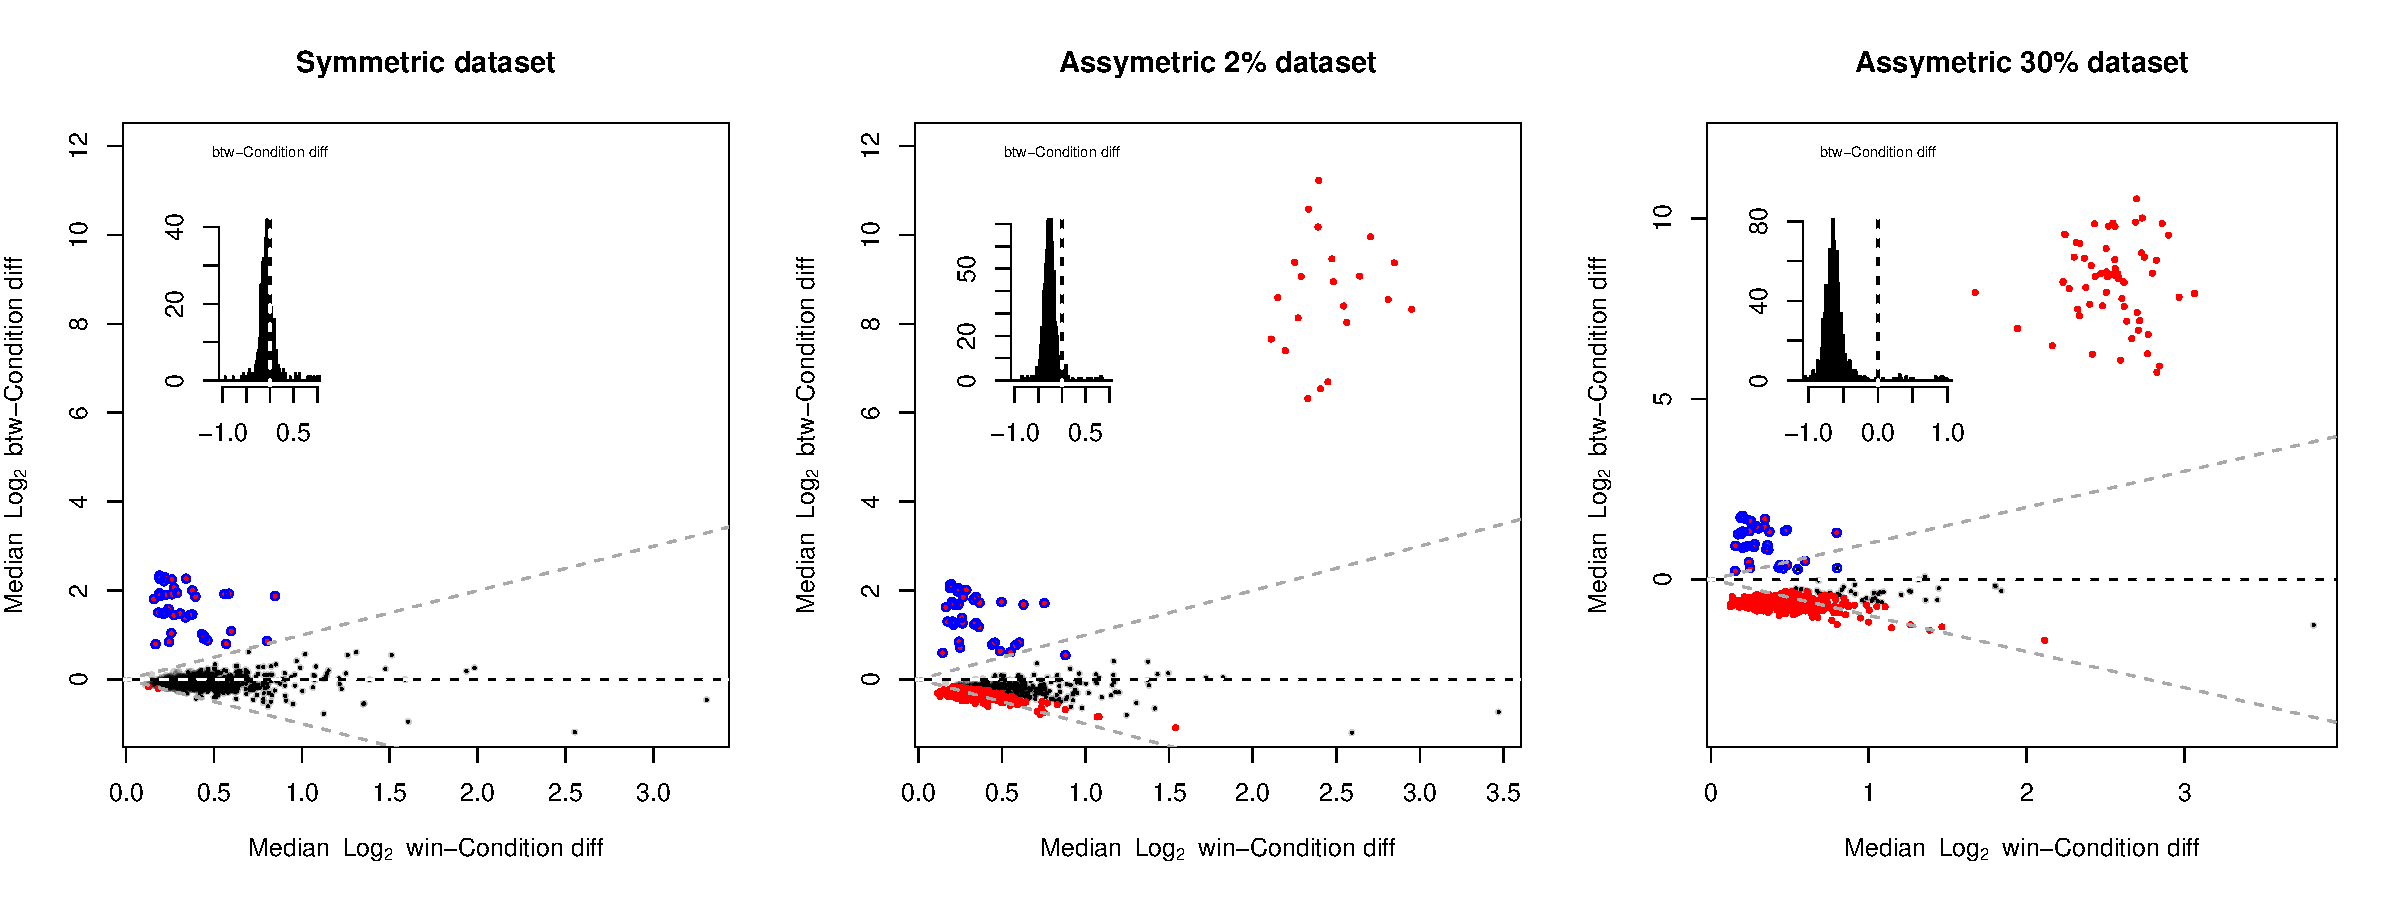
\includegraphics[width=0.9\linewidth]{/Users/ggloor/Documents/0_git/Log-Ratio-Publication/writeup/Fig_1.pdf}
\vspace{3mm} \captionof{figure}{The effect plots \cite{gloor:effect} show the difference between two conditions in simulated RNA-seq datasets with 1000 genes where 40 genes are modelled to have true difference between groups. Each point is a feature (gene), they are coloured in black if not different between groups, red if significantly different between groups, and red with a blue circle if they are one of the 40  genes modelled to be  true positives. The red points in the top right quadrant are the genes modelled to be asymmetrically variable between groups. The inset histograms show the distribution of the differences between groups as calculated by ALDEx2, and the vertical line shows a difference of 0. These x-axis of these plots are truncated to show only differences near the midpoint. The centre of the dataset must be on 0 to prevent the inclusion of false positive and the exclusion of false negative differential abundance identifications.}
\end{center}\vspace{-1cm}

\subsection*{Proposed alternative denominators}
In all cases the geometric mean of the set of features is used and substituted for $g(x)$ in equation 1.
\begin{enumerate}
\item{\textbf{all}} This is the entire set of features; i.e., the CLR
\item{\textbf{IQLR}} This is the set of features that have variance in the dataset between the first and last quartiles 
\item{\textbf{zero}} This is the set of non-zero features in group A, or in group B. Groups A and B thus have different sets of features composing their denominators 
\item{\textbf{User}} This is a set of user-defined features. In Figure 2, these features are the ribosomal protein functions. This is conceptually the ALR with a small number of features instead of a single one
\end{enumerate}

\begin{center}\vspace{-0.5cm}
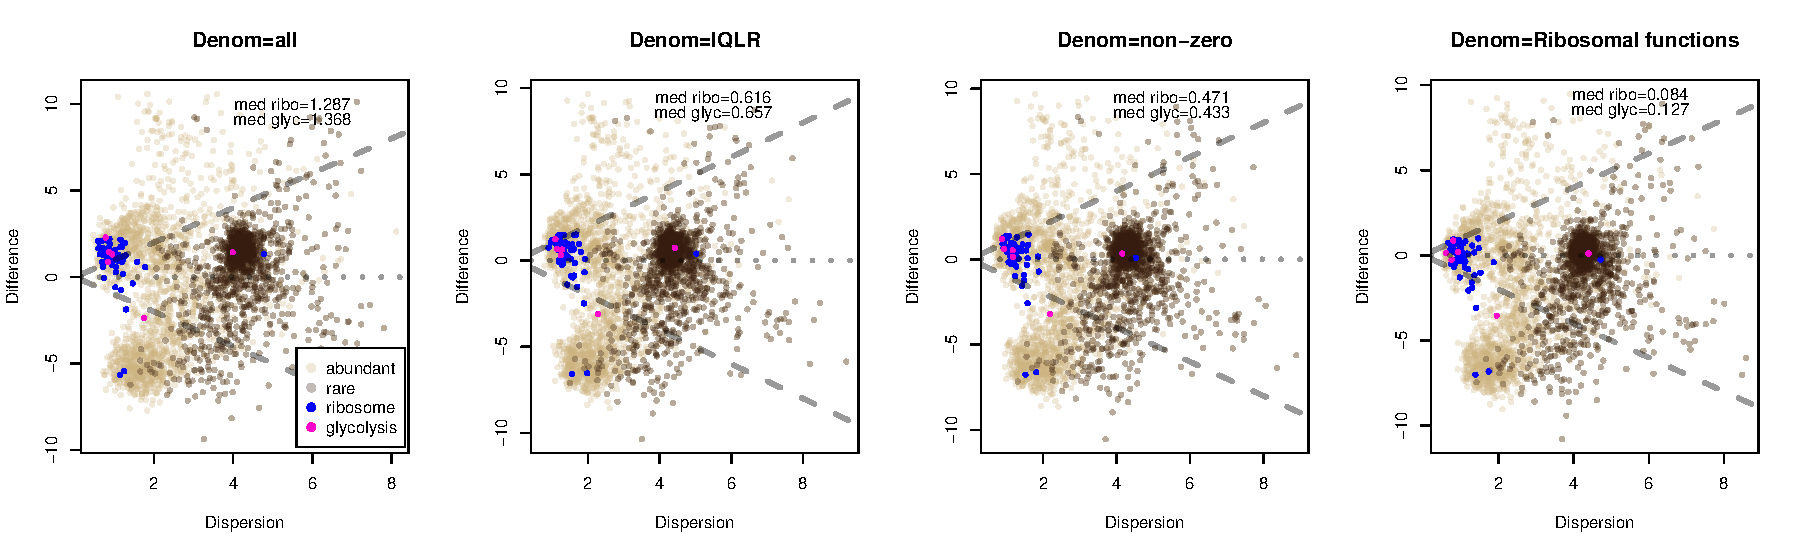
\includegraphics[width=1\linewidth]{/Users/ggloor/Documents/0_git/Log-Ratio-Publication/figures/twtyfr_poster.pdf}
\captionof{figure}{Effect plot and Bland-Altman plots summarizing gene expression in two different states from a meta-transcriptome of health and bacterial vaginosis. Each point is a function, coloured dark brown if rare, light brown if abundant, blue if part of the ribosome, magenta if part of glycolysis. The latter two sets of functions are presumed housekeeping and should be constant between conditions. The mean displacement of these two functional groups is noted. }
\end{center}\vspace{0.0cm}

\begin{center}\vspace{-0cm}
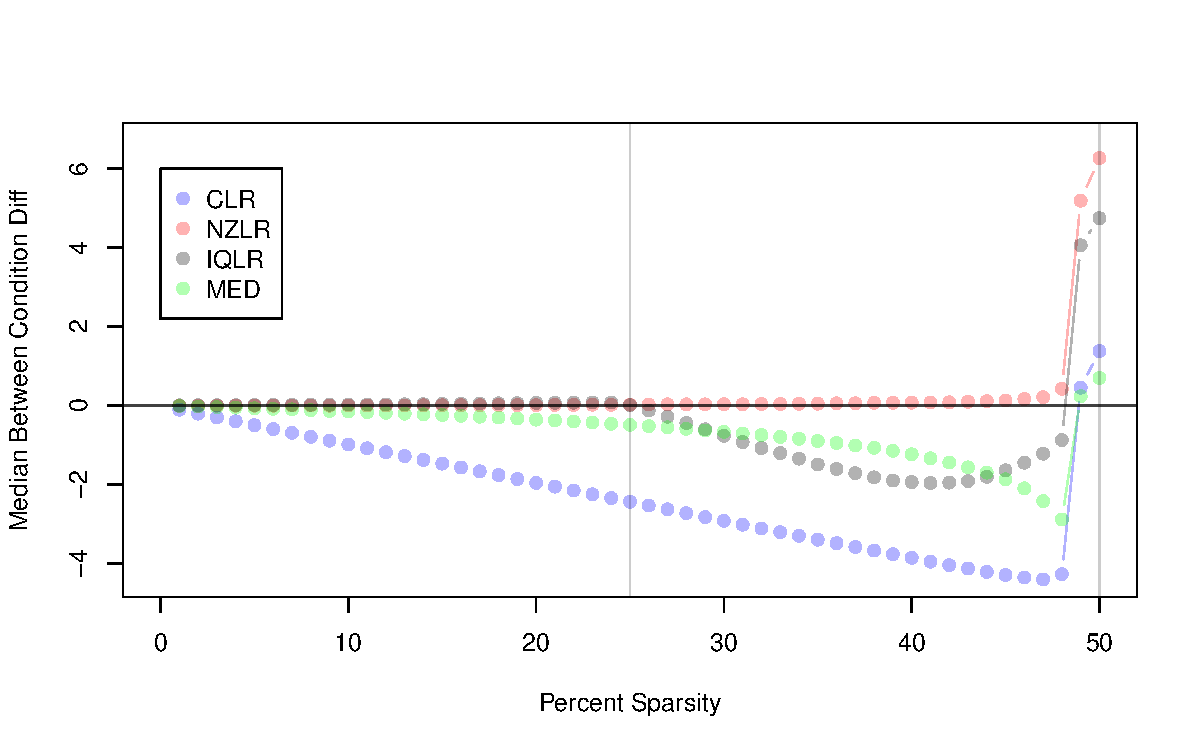
\includegraphics[width=0.6\linewidth]{/Users/ggloor/Documents/0_git/Log-Ratio-Publication/writeup/Fig_failure.pdf}
\captionof{figure}{Each point represents the median between condition difference for a given transformation in a dataset with a specified sparsity. Points closer to the location y=0 are favourable. The CLR transformation fails as soon as asymmetric sparsity is introduced. The IQLR  transformation is effective on datasets with up to 25\% asymmetric sparsity from zeroes or extreme count features. The NZLR transformation is effective on datasets with up to 50\% sparsity . Replacing the geometric mean with the median in Equation 1, is an improvement, but results in a generally small shift in midpoint. }
\end{center}\vspace{0.0cm}

%----------------------------------------------------------------------------------------
%	CONCLUSIONS
%----------------------------------------------------------------------------------------
\vspace{-1cm}
\color{SaddleBrown} % SaddleBrown color for the conclusions to make them stand out

\section*{Conclusions}

\begin{itemize}
\item Asymmetric data is problematic and must be corrected
\item The IQLR approach is the best all purpose starting approach: the zero method is not recommended since sparsity may not be the precipitating issue: in extreme cases such as Figure 2, only a user-defined denominator may be appropriate
\item These approaches have be included in versions of ALDEx2 since 1.6, available on Bioconductor
\end{itemize}

\color{DarkSlateGray} % Set the color back to DarkSlateGray for the rest of the conten %----------------------------------------------------------------------------------------
%	REFERENCES
%----------------------------------------------------------------------------------------
\vspace{-1cm}
\nocite{*} % Print all references regardless of whether they were cited in the poster or not
\bibliographystyle{plain} % Plain referencing style

\bibliography{sample} % Use the example bibliography file sample.bib

%----------------------------------------------------------------------------------------
%	ACKNOWLEDGEMENTS
%----------------------------------------------------------------------------------------
\vspace{-1cm}
\section*{Acknowledgements}

Funded by a grants to GG from the National Science and Engineering Research Council of Canada and Agriculture and Agrifoods Canada
%----------------------------------------------------------------------------------------

\end{multicols}
\end{document}